\documentclass{svproc}
\usepackage[T1]{fontenc}
\usepackage[utf8]{inputenc}
\usepackage{newtxtext,newtxmath}
\usepackage{graphicx,amsmath,float}
\usepackage[hidelinks]{hyperref}
\graphicspath{{../../figures/publication/}}
% Captions for unchanged models, with editorially revised publication labels.
% The simple-story models are experiment-author references, NOT generator outputs.
\newcommand{\HumptyCaption}{Humpty Dumpty: repair attempt, effective repair and remaining damage. Author reference model for the controlled adaptation. Damage is removed only when an attempt and an effective method accompany initial damage; failed help does not establish universal irreparability. The displayed rules were added by the experiment author (sentences S4--S6), with independently settable fall, attempt and method inputs (S7). In the factual setting $F=A=1$, $E=0$, so $R=0$ and $Y=1$. Setting $E=1$ permits repair, but jointly setting $A=0$ leaves damage. These specified counterfactuals are not established by the traditional tale.}

\newcommand{\WolfCaption}{The Boy Who Cried Wolf: credibility and warning are distinct requirements for timely help. Author reference model for the controlled adaptation. A warning is issued in the factual episode, but distrust blocks response. Under the added rules (S3--S6), removing earlier false alarms prevents harm only if the later warning is still given. Harm therefore returns under the joint intervention $\mathrm{do}(F=0,N=0)$. Timely help is assumed to prevent harm completely within this adaptation; the natural retelling does not establish that guarantee. All factual inputs are one, with $V=0$ and $H=1$.}

\newcommand{\CrowCaption}{The Crow and the Pitcher: raising water and already being able to reach it are alternative routes to drinking. Author reference model for the controlled adaptation. The added rules (S3--S6) require an intact pitcher for retained access, but do not make stones universally necessary: $\mathrm{do}(A=0,B=1)$ still yields drinking. Sufficient water and readiness to drink are fixed background conditions. Factually $I=S=1$, $B=0$; adding enough stones raises the water and makes it reachable. The equations specify a controlled Boolean scenario, not a claim that the traditional tale determines every counterfactual.}

\newcommand{\BlackwaterCaption}{Blackwater: fuel, ignition and exposed ships converge on severe fleet fire losses. Codex-assisted narrative hypothesis from television evidence, with unchanged v4 scenario functions. The local view distinguishes Tyrion's control of wildfire from its deployment and his signal from Bronn's ignition; it does not by itself explain the whole battle's winner. Solid arrows denote explicit directional evidence in the retained assistant audit, dashed arrows contextual interpretation. The conjunction and the deployment/response rules are modeling assumptions, not functions identified by the passages. Evidence: S02E05 scene 15; S02E09 scenes 12, 14--16 and 19 in the source register. Independent researcher adjudication remains pending.}

\newcommand{\RedWeddingCaption}{The Red Wedding: prepared attackers and present leaders converge on the hall ambush. Codex-assisted narrative hypothesis, with unchanged v4 functions. Tywin's assurances are interpreted as reducing \emph{Frey's perceived risk in betraying Robb}, not reducing the danger that Robb will be betrayed. Two assumed plot mechanisms differ on whether Walder's grievance is necessary; the guest-attendance conjunction is also an assumption. This view ends at the hall attack, not the destruction of the entire coalition. Solid/dashed arrows distinguish explicit/contextual directional support in the assistant audit. Evidence: S03E06 scene 9; S03E09 scenes 1, 16--17; S03E10 scene 4 (a retrospective report). Independent researcher adjudication remains pending.}

\newcommand{\BoltonCaption}{The Bolton campaign: relief can break an enclosure, yet its necessity for victory depends on the advance mechanism. Codex-assisted narrative hypothesis with unchanged v4 functions. (a) The encirclement mechanism; $H=0$ factually because timely relief arrives. Solid/dashed arrows denote explicit/contextual directional support. (b) Winterfell capture under the full archived model, not just the displayed local slice. With field force $G$, pursuit $P$ and breaching capability $W$, both alternatives use $K=P\land W$ and $Y=K\land P$. ``Relief required'' uses $P=G\land R\land\neg H$; ``untrapped advance'' uses $P=G\land\neg H$. The joint removal of Rickon bait and relief distinguishes them. These are conditional scenarios; the evidence-only partial family leaves all three answers unresolved. Evidence: S06E05 scene 2, S06E09 scenes 9--10 and retrospective S06E10 scene 55. Independent adjudication remains pending.}

\newcommand{\AstaporCaption}{Astapor: command transfer, armed victory and the choice to remain are distinct steps toward departure with freed troops. Codex-assisted narrative hypothesis with unchanged v4 scenario functions. (a) Acquisition of command; (b) attack, emancipation and departure. Repeated $C$ denotes the same variable in both panels. All 12 dependencies are retained. The alternatives differ on whether killing Kraznys is necessary to break the masters' immediate armed control ($S$); the remaining displayed rules also add assumptions. Solid/dashed arrows distinguish explicit/contextual directional support in the assistant audit. The outcome is immediate departure, not durable governance of Astapor. Evidence: S03E03 scene 16 and S03E04 scenes 23--25. Independent researcher adjudication remains pending.}

\typeout{PUBLICATION-TEXTWIDTH: \the\textwidth}
\typeout{PUBLICATION-TEXTHEIGHT: \the\textheight}
\begin{document}
\mainmatter
\raggedbottom
% Include at natural 122-mm width. Do not scale to a narrow two-column slot.
\begin{figure}[H]\centering
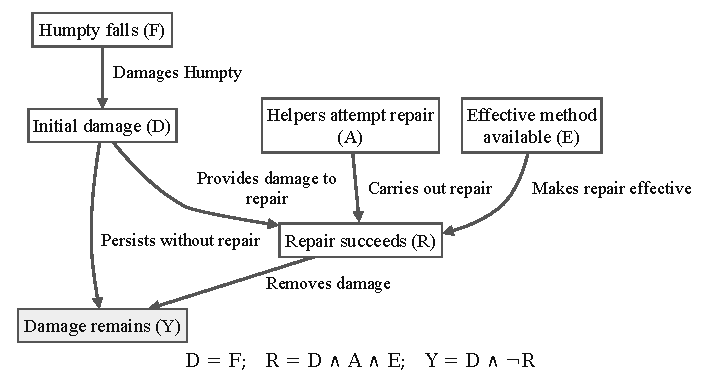
\includegraphics[width=\linewidth]{simple_stories/humpty.pdf}
\caption{\HumptyCaption}\label{fig:pub-humpty}
\end{figure}
\clearpage
\begin{figure}[H]\centering
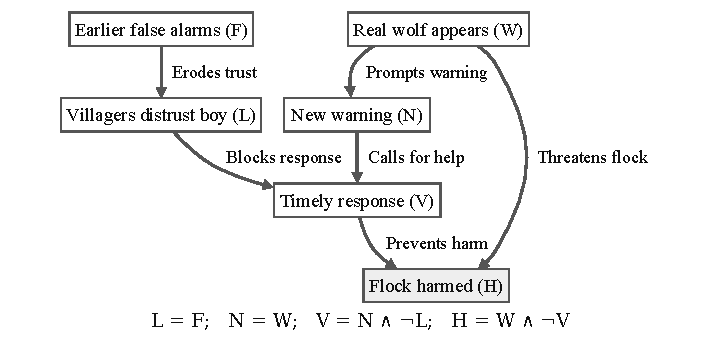
\includegraphics[width=\linewidth]{simple_stories/wolf.pdf}
\caption{\WolfCaption}\label{fig:pub-wolf}
\end{figure}
\clearpage
\begin{figure}[H]\centering
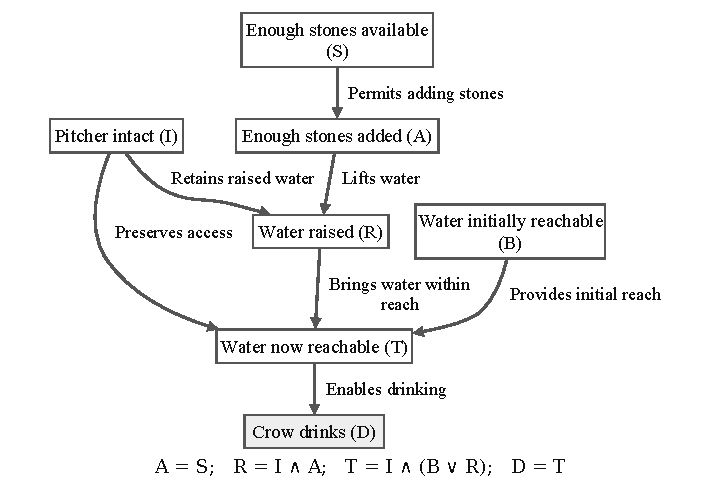
\includegraphics[width=\linewidth]{simple_stories/crow.pdf}
\caption{\CrowCaption}\label{fig:pub-crow}
\end{figure}
\clearpage
\begin{figure}[H]\centering
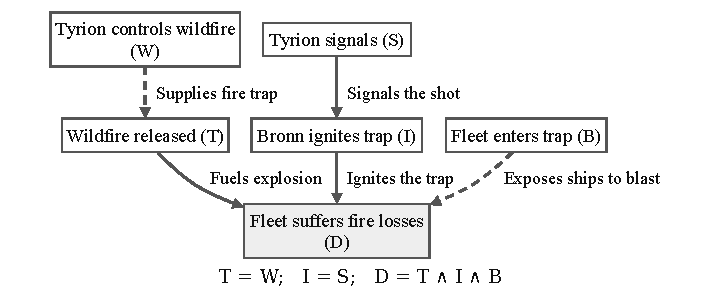
\includegraphics[width=\linewidth]{got/blackwater_mechanism.pdf}
\caption{\BlackwaterCaption}\label{fig:pub-blackwater}
\end{figure}
\clearpage
\begin{figure}[H]\centering
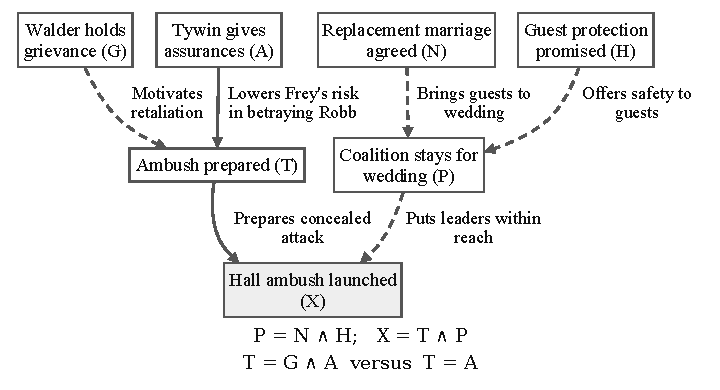
\includegraphics[width=\linewidth]{got/red_wedding_mechanism.pdf}
\caption{\RedWeddingCaption}\label{fig:pub-red-wedding}
\end{figure}
\clearpage
\begin{figure}[H]\centering
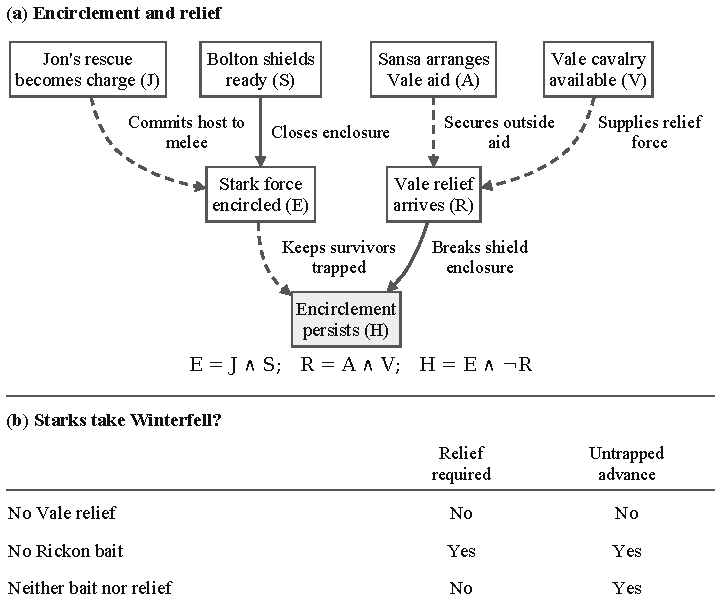
\includegraphics[width=\linewidth]{got/bolton_mechanism_interventions.pdf}
\caption{\BoltonCaption}\label{fig:pub-bolton}
\end{figure}
\clearpage
\begin{figure}[H]\centering
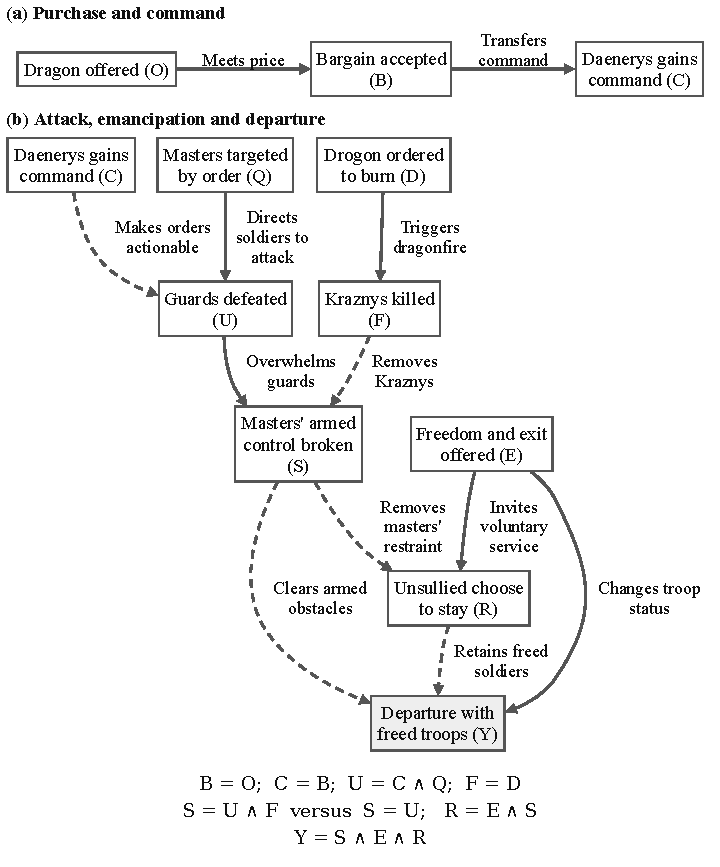
\includegraphics[width=\linewidth]{got/astapor_overview.pdf}
\caption{\AstaporCaption}\label{fig:pub-astapor}
\end{figure}
\end{document}
